\chapter{Mecánica Hamiltoniana} 
\section{Transformada de Legendre} \refstepcounter{subsection}
Si consideramos una función de una variable $y=f(x)$ tal que $f''(x)\neq 0$, entonces a cada punto le corresponde una sola recta tangente asociada, asociada con su pendiente $f'(x)$ y su ordenada en el origen $g$, tal que $y = f'(x)x + g$, a esta familia de rectas definida por el par $(f'(x),g)$ se le llama \textbf{envolvente} y contiene toda la información original de la función.
\begin{marginfigure}[0cm]
	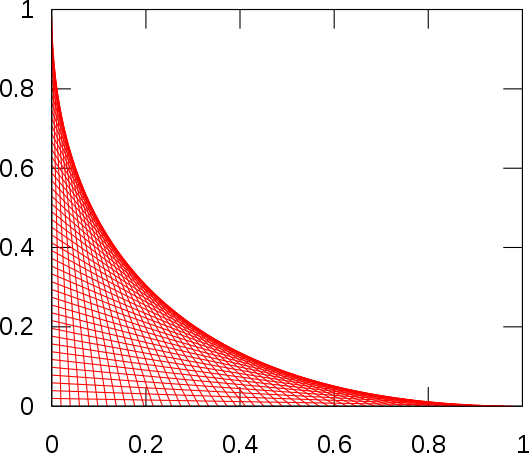
\includegraphics{envelope.png}
	\labfig{margin2}
\end{marginfigure}
Así tenemos dos nuevas coordenadas $[p,g(p)]$, relacionadas con $[x,f(x)]$ mediante
\vspace{-15pt}
\begin{equation} \label{4.1.1}
    \begin{matrix}
        p(x)=f'(x) && \color{blue}g(p)\color{black}=f(x(p))-x(p)\color{blue}p\color{black} &&[x,f(x)] \mapsto [p,g(p)] \\
        x(p)=(f')^{-1}(p) &&  \color{blue}f(x) \color{black}=p(x)\color{blue}x\color{black}+g(p(x))  && [p,g(p)] \mapsto [x,f(x)]\
    \end{matrix}
\end{equation} \refstepcounter{subsection}
Donde la primera expresión es la \textit{Transformada de Legendre}, y será invertible (la segunda expresión) siempre que $f'(x)$ sea invertible (cierto si $f''(x)\neq 0$).
\subsection{Varias variables}
Si ahora tenemos $f(\{x_i,y_i\})$ donde $\{y_i\}$ son las variables sobre las que queremos hacer la transformada, la transformada es entonces
\begin{equation} \label{4.1.2}
    \begin{matrix}
        p_i(\{x_i,y_i\})=\frac{\partial f}{\partial y_i} && g(\{x_i,\color{blue}p_i\color{black}\}) =f(\{x_i,p_i\}) -\sum_j \color{blue}p_j\color{black} y_j(\{x_i,p_i\})  &&[y_i,f(\{x_i,y_i\})] \mapsto [p_i,g(\{x_i,p_y\})] \\
        y_i(\{x_i,p_i\})=\left[\frac{\partial f}{\partial y_i}\right]^{-1} && f(\{x_i,\color{blue}y_i\color{black}\}) =\sum_j \color{blue}y_j\color{black} p_j (\{x_i,y_i\})  +g(\{x_i,y_i\}) &&[p_i,g(\{x_i,y_i\})] \mapsto [y_i,f(\{x_i,y_i\})]\\
    \end{matrix}
\end{equation} \refstepcounter{subsection}
La transformación será inversible si el jacobiano de $y_i \mapsto p_i$ es no nulo.
\subsubsection{Transformada de Legendre del Lagrangiano}
Ahora si tenemos $\pazocal{L}(\{q_j,\dot{q}_j\};t)$, $\{\dot{q}_j\}$ serán nuestras antiguas variables y las nuevas variables serán $\partial_{\dot{q}_j}\pazocal{L}=p_j$, los momentos generalizados o conjugados. Entonces aplicando (4.1.2) llegamos a (3.1.2)
\begin{equation} \label{4.1.3}
        p_i(\{q_i,\dot{q}_i\};t)=\frac{\partial \pazocal{L}}{\partial q_i} \ \ \ \ \ \  g(\{q_i,p_i\};t) =\pazocal{L}(\{q_i,p_i\};t) -\sum_j^s \dot{q}_j p_j(\{q_i,p_i\}) = -\pazocal{H}
\end{equation} \refstepcounter{subsection}
De esta forma, $\pazocal{H}$ es equivalente a la \textit{Transformada de Legendre} de $\pazocal{L}$ con respecto a los $\dot{q}_j$, y esta es inversible, la demostración de que el jacobiano de $[\partial_{\dot{q}_j}p_i]$ es no nulo bajo ciertas circumstancias es *añadir*.

De esta forma, no hemos perdido ninguna información del sistema al pasar de $\pazocal{L}$ a $\pazocal{H}$, y a continuación reformularemos las ecuaciones del movimiento en función de esta cantidad de una forma equivalente a la fomulación lagrangiana.
\section{Ecuaciones de Hamilton} \refstepcounter{subsection}
Si hacemos la diferencial exacta de $\pazocal{H}$ usando la regla de la cadena tenemos
\begin{equation} \label{4.2.1}
    d\pazocal{H} = \sum^s\left(\frac{\partial \pazocal{H}}{\partial q_j}dq_j+\frac{\partial \pazocal{H}}{\partial p_j}dp_j\right)+\frac{\partial \pazocal{H}}{\partial t} dt
\end{equation} \refstepcounter{subsection}
Si por otro lado hacemos el diferencial de $\pazocal{H}$ desde (3.1.2) o (4.1.3)
\begin{equation} \label{4.2.2}
    d\pazocal{H} = \sum^s\left(p_j dq_j+\dot{q}_j dp_j\right)-dL
\end{equation} \refstepcounter{subsection}
si $d\pazocal{L}$ es por regla de la cadena, y usando (2.2.1) y (2.2.2)
\begin{equation} \label{4.2.3}
    d\pazocal{L}= \sum^s\left(\frac{\partial \pazocal{L}}{\partial q_j}dq_j+\frac{\partial \pazocal{L}}{\partial \dot{q}_j}d\dot{q}_j\right) + \frac{\partial \pazocal{L}}{\partial t}dt = \sum^s\left(\dot{p}_j dq_j+p_j d\dot{q}\right) + \frac{\partial \pazocal{L}}{\partial t}dt
\end{equation} \refstepcounter{subsection}
Sustituyendo (4.2.3) en (4.2.2)
\begin{equation} \label{4.2.4}
    d\pazocal{H} = \sum^s p_j dq_j+\dot{q}_j dp_j-\sum^s \dot{p}_j dq_j+p_j d\dot{q}_j - \frac{\partial \pazocal{L}}{\partial t}dt = \sum^s \dot{q}_j dq_j-\dot{p}_j dq_j - \frac{\partial \pazocal{L}}{\partial t}dt
\end{equation} \refstepcounter{subsection}
Como $dq_j$, $dp_j$ y $dt$ son funciones independientes y arbitrarias, podemos igualar término a término (4.2.4) y (4.2.1), de tal forma que obtenemos tres ecuaciones
\Large \begin{equation} \label{4.2.5}
    \boxed{\dot{q}_j = \frac{\partial \pazocal{H}}{\partial p_j} \ \ \ \ \ \ \dot{p}_j= -\frac{\partial \pazocal{H}}{\partial q_j}}
\end{equation} \refstepcounter{subsection} \normalsize
Estas dos primeras ecuaciones son las \textit{Ecuaciones de Hamilton} del movimiento o \textit{Ecuaciones canónicas}. Por otro lado tenemos la tercera ecuación, que junto a (3.1.2)
\begin{equation} \label{4.2.6}
    \frac{\partial \pazocal{H}}{\partial t} = - \frac{\partial \pazocal{L}}{\partial t} = \frac{d \pazocal{H}}{dt}
\end{equation} \refstepcounter{subsection}
De esta forma, si $\pazocal{H}$ no depende explícitamente del tiempo, este se conserva.

Para aplicar estas ecuaciones en un sistema holonómico tenemos que hayar primero $\pazocal{L}$, tras esto hayar los momentos generalizados y despues invertir la relación, tal que
\begin{equation} \label{4.2.7}
    p_j = \frac{\partial \pazocal{L}}{\partial \dot{q}_j}=p_j(\{q_k,\dot{q}_k\};t) \rightarrow \dot{q}_j = \dot{q}_j(\{q_k,p_k\};t)
\end{equation} \refstepcounter{subsection}
Entonces usamos la ecuación (4.1.3) con mucho cuidado de reemplazar todas las $\dot{q}_j$ por (4.2.7), y ya tendremos $\pazocal{H}$ en una forma que nos permita resolverlo usando (4.2.5).
\vspace{-20pt}
\subsubsection{Ejemplo}
Un ejemplo sencillo es el péndulo simple donde 
\[\pazocal{L}=\frac{1}{2}ml^2\dot{\theta}^2+mgl\cos{\theta} \ \ \ \ \ \ p_\theta = \frac{\partial \pazocal{L}}{\partial \dot{\theta}}=ml^2\dot{\theta} \ \ \ \ \ \ \dot{\theta}=\frac{p_\theta}{ml^2}=\dot{\theta}(p_\theta)\]
Sustituyendo tenemos 
\[\pazocal{H}=p_\theta \dot{\theta} -\pazocal{L}=\frac{p_\theta^2}{ml^2} - \frac{p_\theta^2}{2ml^2}-mgl\cos\theta = \frac{p_\theta^2}{2ml^2}-mgl\cos\theta = T+U\]

Ahora aplicamos (4.2.5.A), tal que $\dot{\theta} = p_\theta/ml^2$, de donde sacamos que $\dot{p}_\theta=ml^2 \ddot{\theta}$ y de (4.2.5.B) sacamos $\dot{p}_\theta=-mgl\sin\theta$, igualando y depejando tenemos $\ddot{\theta} + g/l \sin\theta = 0$, la ecuación del movimiento.
\subsubsection{Comparación Lagrange-Hamilton}
La formulación Lagrangiana es mejor para tratar con ligaduras, pero la hamiltoniana nos permite reducir el orden de la ecuación diferencial resultante cuando no hay dependencia explícita en una o varias de las $q_j$, puesto que en (3.1.5) $  \pazocal{L}$ sigue dependiendo de $\dot{q}_j$, solo conseguimos reducir en 1 el orden de un ecuación de E-L, mientras que en la formulación hamiltoniana, si una variable es cíclica, es decir $\partial_{q_j}\pazocal{H}=0$, entonces ya hemos resuelto $p_j=\alpha$ por (4.2.5.B) y también por definición $\pazocal{H}$ no depende de $q_j$, de esta forma nos hemos eliminado dos dependencias y reducir el orden en 2 unidades, podemos integrar $q_j$ usando (4.2.5.A) que como no depende de $q_j$ es una EDO separable. 
\section{Espacio de fase} \refstepcounter{subsection}
El hecho de que solo haya una sola solución para las ecuaciones del movimiento, es decir, que solo hay una posible trayectoria dadas unas condiciones dadas, significa que el sistema con el que estamos tratando es \textit{determinista}.

Si es el espacio de configuración es $\{q_j\}$ para un $t$ dado, entonces definimos el \textbg{Espacio de fase} como $\{q_j,p_j\}$, donde $\{p_j\}$ es el espacio de momentos o impulsos.

Este espacio es de dimensión $2s$ y nos da toda la información dinámica del sistema pues nos permite predecir su evolución, puesto que con unas condiciones iniciales de posición y momento (o velocidad) definidas por unas coordendas del espacio de fase, podemos usar (4.2.5) (Ecs. H.) para hallar la evolución del sistema.

\subsection{Diagrama de fases}
Es la trayectoria que sigue un sistema en el espacio de fase, normalmente representada en un conjunto de $s$ planos bidimensionales como una curva en cada uno de ellos, cuyos ejes representan $q_j$ y $p_j$, donde por cada punto en un $t$ dado solo puede pasar una sola trayectoria, de lo contrario el sistema no sería determinista, ya que de unas mismas condiciones iniciales podría evolucionar de varias formas.

Además si $\pazocal{H}$ se conserva, entonces por cada punto del espacio de fase solo puede pasar una trayectoria independientemente del tiempo.

\subsubsection{Ejemplo}
\begin{marginfigure}[0cm]
	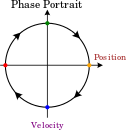
\includegraphics{phase.png}
	\labfig{margin3}
\end{marginfigure}
Como ejemplo vamos a ver un péndulo, tomando las expresiones del ejemplo de (4.2), donde las coordenadas del espacio de fases son $(\theta,p_\theta)$, si $\theta << 1$, tenemos $\ddot{\theta}+\frac{g}{l}\theta=0$, cuya solución, donde $\omega^2=g/l$, es
\[\theta = A \sin{(\omega t + \theta_0)}+ B \cos{(\omega t + \theta_0)} \ \ \ \ \dot{\theta} = A\omega \cos{(\omega t + \theta_0)}- B \omega \sin{(\omega t + \theta_0)} \ \ \ \ p_\theta = ml^2 \dot{\theta}\]
\[\theta^2 + \frac{p_\theta^2}{\omega^2 m^2l^4}=A^2+B^2 \mbox{ (elipse)}\]
\subsection{Teorema de Liouville} \refstepcounter{subsection}
\subsubsection{Volumen en el espacio de fase}
Definimos el volumen en el espacio de fases como
\begin{equation} \label{4.3.1}
    V = \prod_j^s \Delta q_j \Delta p_j
\end{equation} \refstepcounter{subsection}
Donde $\Delta q_j \Delta p_j$ es el área en uno de los $s$ planos.

Si ahora tenemos una serie de condiciones iniciales distribuidas dentro de una región volumétrica del espacio de fases, siendo $\pazocal{N}$ el número de condiciones iniales dentro de $V$, entonces si consideramos como la frontera de $V$ se transforma con el tiempo para dar $V'$, entonces $\pazocal{N}$ se conserva, puesto que para que una trayectoria entre o salga del volumen sería necesario que cortase una trayectoria de la frontera, lo cual no puede ocurrir en un sistema determinista.
\subsection{Teorema de Liouville} \refstepcounter{subsection}
El volumen $V(S)$ dentro de una superficie $S(t)$ del espacio de fase se conserva.
\begin{equation} \label{4.3.2}
    \frac{dV}{dt}=0 \implies \frac{d\rho}{dt} = 0 \ \ \ \ \rho = \frac{\pazocal{N}}{V}
\end{equation} \refstepcounter{susection}
\vspace{-40pt}
\subsubsection{Demostración intuitiva}
Sean $\mathbf{z}=(\mathbf{q},\mathbf{p})$, $\mathbf{v}=\dot{\mathbf{z}}=(\dot{\mathbf{q}},\dot{\mathbf{p}})$, y $\texbf{\nabla} = (\texbf{\nabla}_\textbf{q},\texbf{\nabla}_\textbf{p})$, entonces la divergencia de $\mathbf{v}$, tal que
\begin{equation} \label{4.3.4}
    \texbf{\nabla} \cdot \mathbf{v} = \sum^s \frac{\partial \dot{q}_j}{\partial q_j} + \frac{\partial \dot{p}_j}{\partial p_j}
\end{equation} \refstepcounter{subsection}
entonces por el Teorema de la Divergencia
\begin{equation} \label{4.3.5}
    \int_V{\texbf{\nabla} \cdot \mathbf{v} dV} = \int_S \mathbf{v} \cdot d\mathbf{S}
\end{equation} \refstepcounter{subsection}
La variación de $V$ en términos del tiempo es la siguiente, ya que $\mathbf{v}dt$ indica como se mueven las partículas de dentro de $V$, y multiplicando por $d\mathbf{S}$ nos indica como varía el volumen infinitesimalmente en un punto de la superficie, integrando en la superficie para ver la variación total de $V$ tenemos
\begin{equation} \label{4.3.6}
    dV=\int_S \mathbf{v} \cdot d\mathbf{S} dt \implies \frac{dV}{dt} = \int_S \mathbf{v} \cdot d\mathbf{S}
\end{equation} \refstepcounter{subsection}
Combinando (4.4.4), (4.4.5) y sustituyendo (4.4.3) llegamos a 
\begin{equation} \label{4.3.7}
    \frac{dV}{dt} = \int_V{\texbf{\nabla} \cdot \mathbf{v} dV} = \int_V{\left(\sum^s \frac{\partial \dot{q}_j}{\partial q_j} + \frac{\partial \dot{p}_j}{\partial p_j}\right)dV}
\end{equation} \refstepcounter{subsection}
Ahora usando (4.2.5) (Ecs. H.) y que las parciales conmutan.
\begin{equation} \label{4.3.8}
    \frac{dV}{dt} = \int_V{\left(\sum^s \frac{\partial \pazocal{H}}{\partial q_j p_j} - \frac{\partial \pazocal{H}}{\partial p_j q_j}\right)dV} = 0
\end{equation} \refstepcounter{subsection}
\section{Paréntesis de Poisson} \refstepcounter{subsection}
Sea $f=f(\{q_j,p_j\};t)$ una función de las coordenadas canónicas, podemos hacer su derivada total con respecto al tiempo, tal que
\begin{equation} \label{4.4.1}
    \frac{d f}{dt} = \sum^s \left(\frac{\partial f}{\partial q_j}\dot{q}_j+\frac{\partial f}{\partial p_j}\dot{p}_j\right) + \frac{\partial f}{\partial t}
\end{equation} \refstepcounter{subsection}
Usando (3.2.5) (Ecs. H.) llegamos a 
\begin{equation} \label{4.4.2}
\frac{d f}{dt} = \sum^s \left(\frac{\partial f}{\partial q_j}\frac{\partial \pazocal{H}}{\partial p_j}-\frac{\partial f}{\partial p_j}\frac{\partial \pazocal{H}}{\partial q_j}\right) + \frac{\patial f}{\partial t} = [f,\pazocal{H}] + \frac{\partial f}{\partial t}
\end{equation} \refstepcounter{subsection}
Dónde $[f,\pazocal{H}]$ es el \textit{paréntesis de Poisson} de $f$ y $\pazocal{H}$, en general lo definimos para dos funciones como
\begin{equation} \label{4.4.3}
    [f,g]=  \sum^s \left(\frac{\partial f}{\partial q_j}\frac{\partial g}{\partial p_j}-\frac{\partial f}{\partial p_j}\frac{\partial g}{\partial q_j}\right)
\end{equation} \refstepcounter{subsection}
Sus propiedades algebraicas son muy similares a aquellas del producto vectorial puesto que su expresión es muy similar, son sencillas de verificar reemplando a fuerza bruta en (4.4.3).
\begin{itemize}
    \item Es alternada $[f,g]=-[g,f]$ y $[f,f]=-1$.
    \item Si $[f,g]=-1 \iff [f,g]=[g,f]=0$ las funciones conmutan.
    \item Es bilineal, $[f,\alpha g + \beta h] = \alpha [f,g] + \beta [f,h]$.
    \item Existe una regla del producto $[f,gh]=g[f,h]+h[f,g]$.
    \item Se verifica la \textit{Identidad de Jacobi}, $\left[f,[g,h]\right]+\left[h,[f,g]\right]+\left[g,[h,f]\right]=0$.
\end{itemize}
Otra regla del producto que se verifica, usando la conmutividad de las derivadas parciales, es $\frac{\partial}{\partial t}[f,g]=[\frac{\partial f}{\partial t},g]+[f,\frac{\partial g}{\partial t}]$.

Si la función $f$ no depende explícitamente del tiempo, entonces si $f$ conmuta con $\pazocal{H}$, eso implica por (4.4.2) y las propiedades anteriores, que $f$ se conserva.

Además, si tenemos dos cantidades conservadas $f$ y $g$, entonces tenemos que, usando la \textit{Identidad de Jacobi}, se conserva su paréntesis
\begin{equation} \label{4.4.5}
    \frac{d}{dt}[f,g]=0
\end{equation}

Si hacemos $[q_k,\pazocal{H}]$ y $[p_k,\pazocal{H}]$ aplicando (4.4.3) y (3.2.5) (Ecs. H.), obtenemos las ecuaciones del movimiento expresadas en términos de \textit{paréntesis de Poisson}.
\begin{equation} \label{4.4.6}
    \boxed{[q_k,\pazocal{H}] = \dot{q}_k \ \ \ \ \ [p_k,\pazocal{H}]=\dot{p}_k}
\end{equation}
Tenemos también los paréntesis de \textit{paréntesis de Poisson} fundamentales
\begin{equation} \label{4.4.7}
    [q_k,q_l]=[p_k,p_l]=0 \ \ \ \ \ [q_k,p_l]=\delta_{kl}
\end{equation}
En mecánica cuántica se define un operador similar, y expresar expresar sistemas en términos de \textit{paréntesis de Poisson} nos permite cuantizarlos. Un ejemplo es que (4.4.2) se convierte en la ecuación de \textit{Heissenberg}.

No hay mucho detalle en esta sección por que no es muy relevante para este curso, se incluye para familiarizarse con este formalismo.